\documentclass[journal]{new-aiaa}
%\documentclass[conf]{new-aiaa} for conference papers
%\documentclass{article}
\usepackage[utf8]{inputenc}
\usepackage{textcomp}
\usepackage{svg}
\usepackage{graphicx}
\usepackage{amsmath}
\usepackage[version=4]{mhchem}
\usepackage{siunitx}
\usepackage{longtable,tabularx}
\usepackage{multicol}
\usepackage{geometry} % For custom page size and margins
\usepackage{rsfso}
\setlength\LTleft{0pt} 


% Set custom page size and margins for a total width of 7 inches
%\geometry{
%  letterpaper, 
%  left=0.375in, 
%  right=0.375in, 
%  top=1in, 
%  bottom=1in, 
%  columnsep=0.5in % Space between the two columns
%}


\title{Thermo-mechanical Impact of Thruster Plume Impingement on Space Debris}

\author{Jacob Higgins \footnote{Undergraduate Student, School of Civil, Aerospace, and Design Engineering, jacob.higgins.2021@bristol.ac.uk.}}


\author{Lucy Berthoud \footnote{Professor, School of Civil, Aerospace, and Design Engineering.}}
\affil{University of Bristol Queen's Building, BS8 2TR, United Kingdom}

\author{Fiona Hulton-Harrop \footnote{Senior Thermal Engineer, Astroscale Ltd.}}
\affil{Astroscale Ltd.,Zeus Rutherford Avenue, Harwell Campus, Didcot, Oxfordshire, England, OX11 0DF}

\begin{document}
%\onecolumn
\maketitle

\begin{abstract}
Active debris removal (ADR) is defined as a capability to interact with passive orbiting objects, in order to reduce their orbital lifetime \cite{steeringgroupIADCStatementActive2022a}. It is known that ADR is necessary to control the unstable growth rate of debris in low Earth orbit (LEO)\cite{inter-agencyspacedebriscoordinationcommitteePeacefulUsesOuter1993} \cite{bastidavirgiliActiveDebrisRemoval2013}. Considerable work has been done on assessing the feasibility of active debris removal missions (cite lots here). One proposed method for this is to use plume impingement of a reaction control system (RCS) thruster on the capturing spacecraft. This work looks at the effect of the mechanical and thermal effects of a thruster plume on the debris, in order to assess the risk that this de-tumbling method could cause break-off of material and appendages such as solar panels and antennas. A classification of the severity of different potential debris objects is also presented, in order to quantify this risk of this method, in terms of the likelihood of break-off and the potential impact of the debris.
\end{abstract}


\section*{Nomenclature}

\noindent(Nomenclature entries should have the units identified)

{\renewcommand\arraystretch{1.0}
\noindent\begin{longtable*}{@{}l @{\quad=\quad} l@{}}
$\rho$ & density\\
$p$ & pressure \\
$m$ & mass\\
$T$ & Temperature\\
$\sigma_T$ & collision cross section\\
$\Theta$ & boundary-layer momentum thickness\\
\multicolumn{2}{@{}l}{Subscripts}\\
$E$ & Nozzle exit flow conditions \\
$*$ & Throat flow conditions \\
$0$ & Stagnation flow conditions \\
\end{longtable*}}





%\twocolumn
\section{Introduction}
\label{sec-introduction}


Active debris removal (ADR) is defined as a capability to interact with passive orbiting objects, in order to reduce their orbital lifetime \cite{steeringgroupIADCStatementActive2022a}. It is known that ADR is necessary to control the unstable growth rate of debris in low Earth orbit (LEO) \cite{inter-agencyspacedebriscoordinationcommitteePeacefulUsesOuter1993} \cite{bastidavirgiliActiveDebrisRemoval2013}. Considerable work has been done on assessing the feasibility of active debris removal missions \cite{ledkovReviewContactContactless2022,bonnalActiveDebrisRemoval2013}. It showed that during ADR, it is necessary to minimise the spin rate differential between debris and the capturing spacecraft \cite{shanReviewComparisonActive2016}. One proposed method of for this is to use plume impingement of a reaction control system (RCS) thruster on the capturing spacecraft, to create a moment on the debris \cite{peters2016applicability,ferrariGASPLUMEIMPINGEMENT2014}. 

\subsection{Plume Impingement}

A thruster plume in Earth orbit expands differently to a plume blow the ionosphere, due to the severely low downstream pressure at higher altitudes. Expansion fans at the nozzle exit do not expand according to the Prandtl-Mayer angle, but instead expand more radially as if emanating from a point source at the centre of the nozzle \cite{mehtaUnderexpandedSupersonicPlume2011}. The low downstream pressure also leads to a decreasing mean free path in the plume- defined as the average distance travelled by a particle between successive particular collisions:

\begin{equation}
  \lambda = \frac{m}{\sqrt{2} \rho {\sigma}_T} 
  \label{intro_eq_meanFreePath}
\end{equation}

As $\lambda$ increases, the gas transitions from behaving like a continuum where Navier-Stokes (and all derived flow equations) are valid, to a rarefied gas where instead kinetic theory must be applied to accurately capture the particular nature of the gas \cite{pittPlumeImpingementStudies}. The Knudsen number is commonly used to quantify this transition from continuum to rarefaction \cite{knudsenGesetzeMolekularstromungUnd2006}. This parameter is equal to the mean free path, normalised by a characteristic length. In literature for plume impingement studies, the characteristic length chosen is commonly a nozzle parameter, but can differ between nozzle radius, nozzle diameter, throat radius, and nozzle length \cite{caiGaskineticSolutionsHigh2013,sharmaDSMCSimulationRocket2023,singhalNumericalStudyNozzle2024,subramanianUnderexpandedJetImpingement2024}. Knudsen number is used to split the plume into three regions: continuum region; transition region; and the free molecular region. These regions and the applicable Knudsen number ranges are shown in Figure \ref{intro_fig_FlowRegions}. In the transition region, the gas is neither a continuum or rarefied gas. Often, direct simulation monte carlo (DSMC) computations are used to characterise this region of the flow. In addition, DSMC codes allow for the computation of non-equilibrium thermal balance conditions between a plume and the surface upon which it impinges. Notably, when running DSMC calculations, the distinction between the flow regions from Figure \ref{intro_fig_FlowRegions} is generally determined by Bird's parameter rather than the Knudsen number. Bird's parameter is simply the Knudsen number where the characteristic length is constrained to the cell size of the mesh \cite{birdMolecularGasDynamics2003}. Legge had some success by omitting the transition region, and treating the flow as either continuum or rarefied \cite{leggeModellingControlThruster1982}. Impingement was then calculated in the transition regime by estimating a reduced pressure coefficient: an average of pressure coefficients in the adjacent continuum and free molecular regions. In Legge's case, this averaging was based on experimental data of his specific thruster, and so likely does not constitute a valid general method.




\begin{figure}[ht]
  \centering
  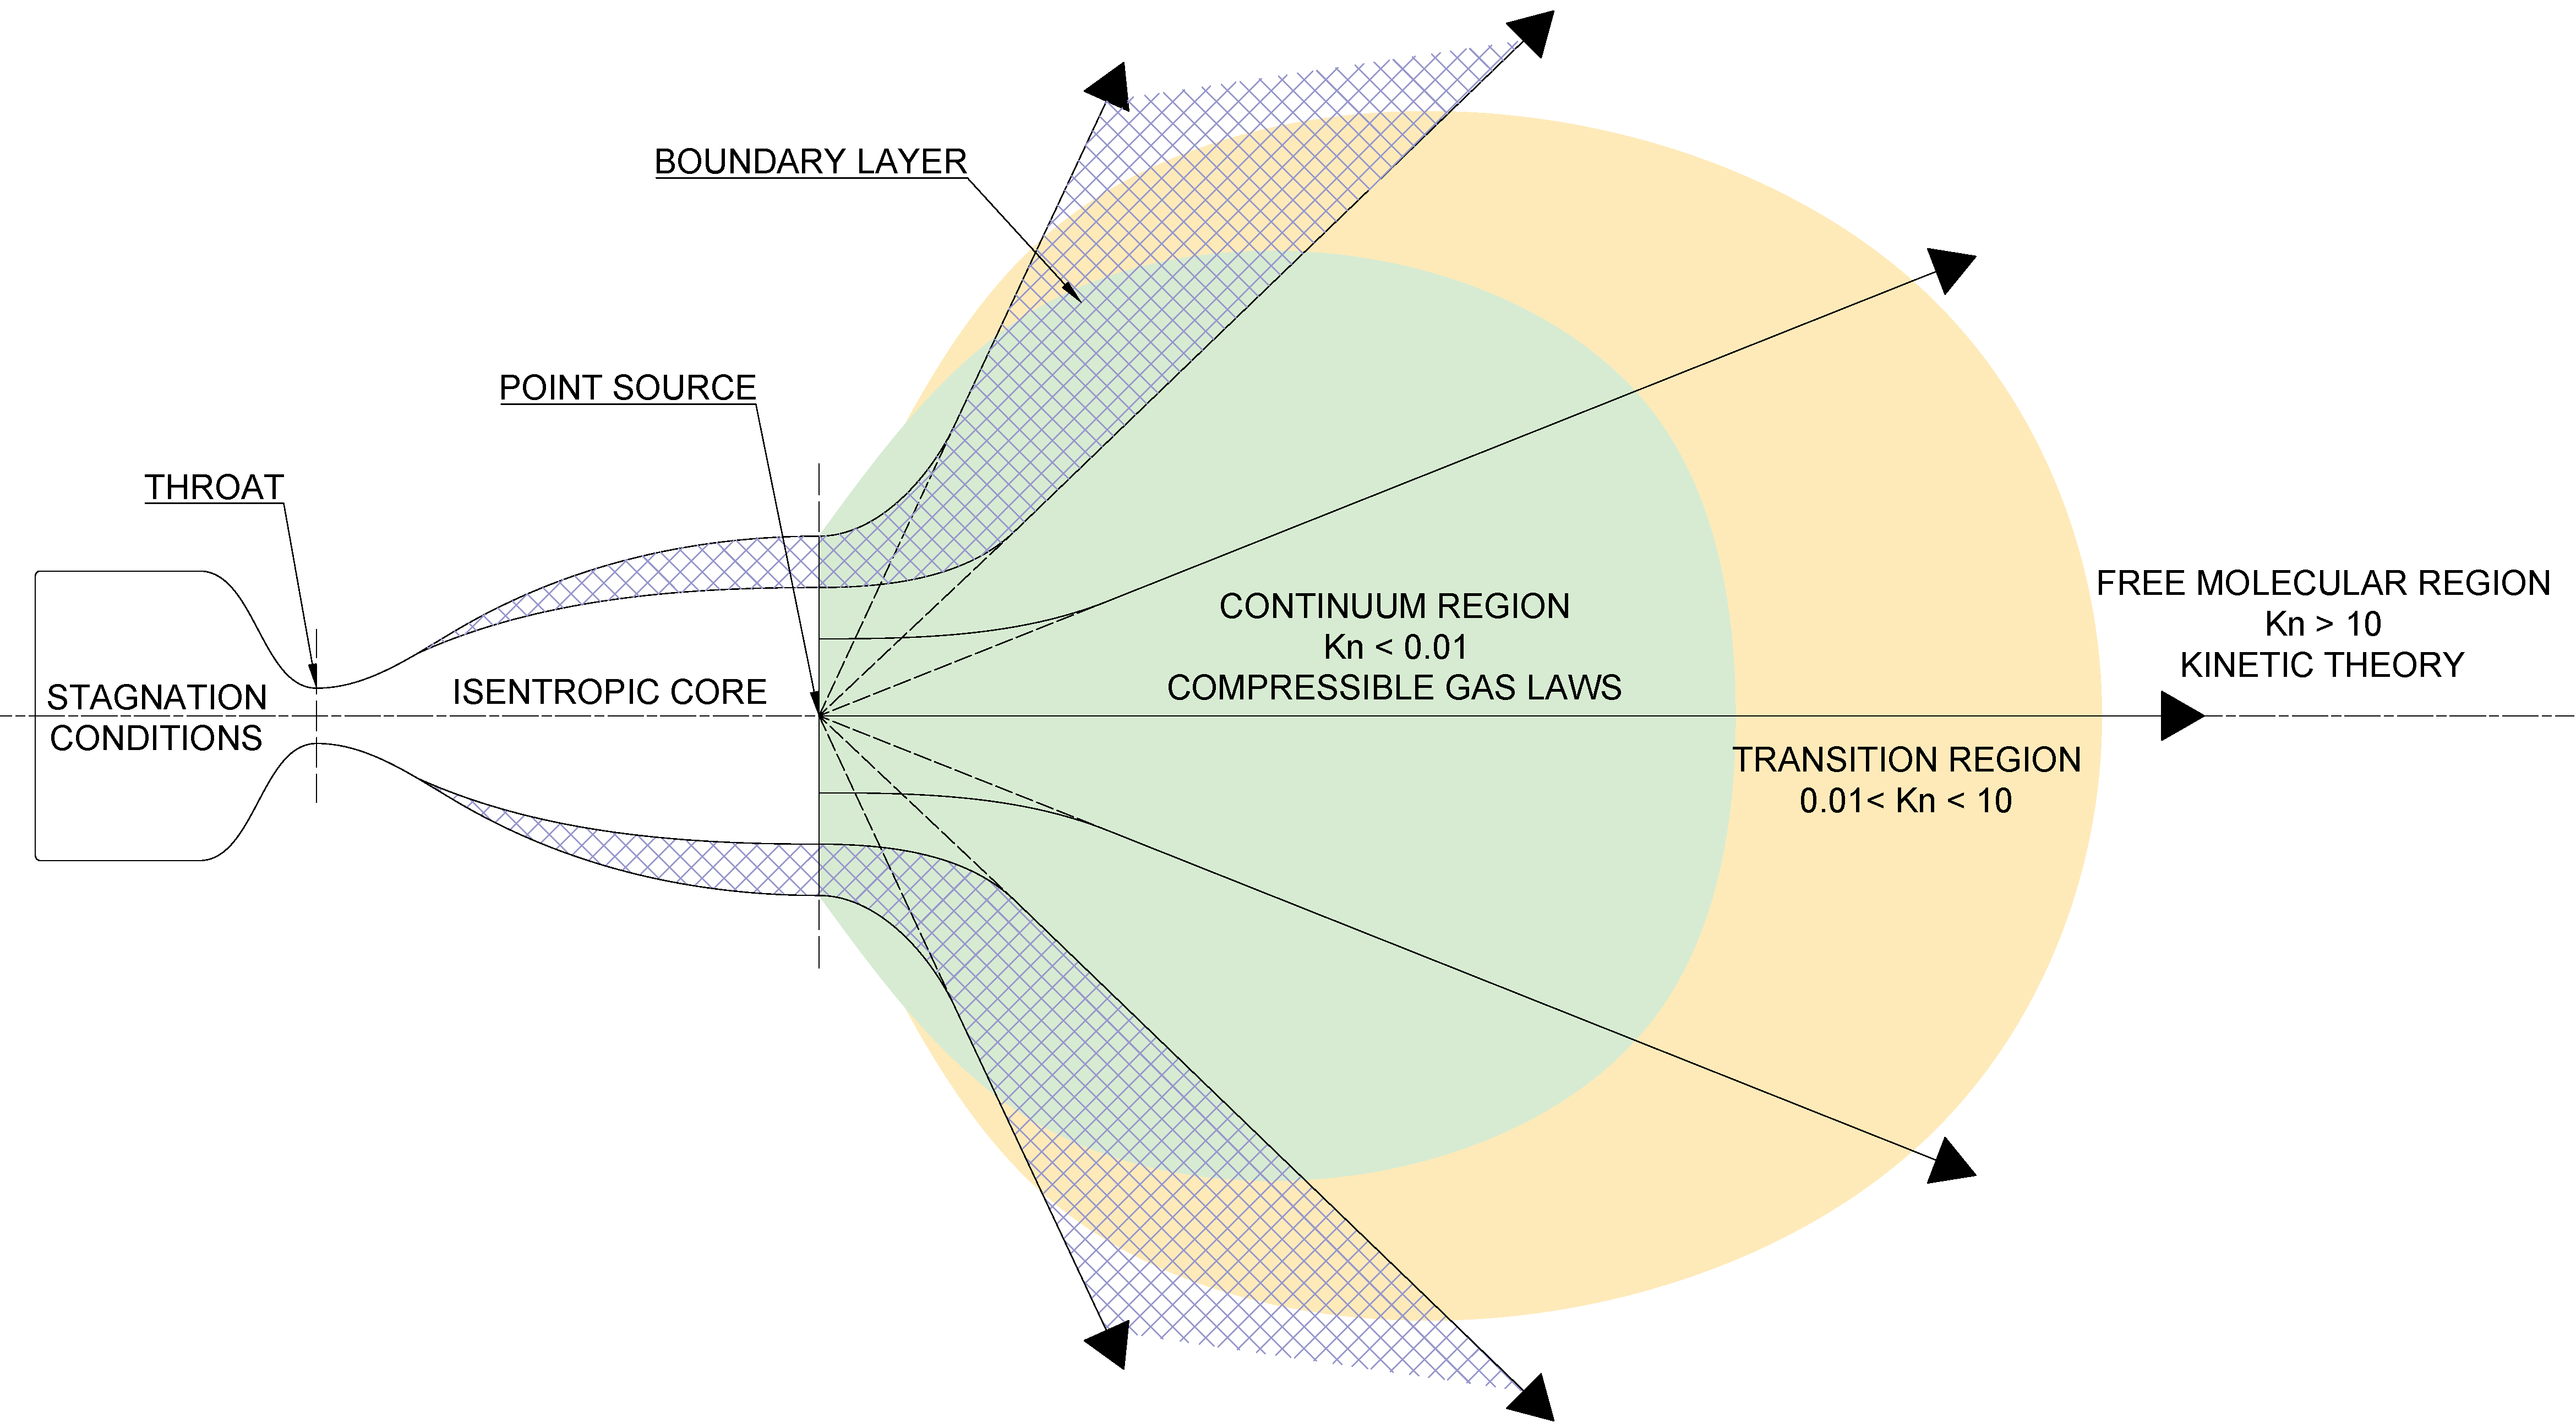
\includegraphics[width=\columnwidth]{Figures/FlowRegions.pdf}
  \caption{Flow Regions from an isentropic nozzle exhaust, and their characteristic Knudsen number ranges.}
  \label{intro_fig_FlowRegions}
\end{figure}

Equation \ref{intro_eq_meanFreePath} shows for a plume with a single particle species A, and hence a constant particular mass and collision cross section, the mean free path is inversely proportional to the density of the plume. Analytical methods for determining the density field of the plume commonly include Simon's model and Mayer's model \cite{simonsEffectNozzleBoundary1972} \cite{mayerThrustLossDue1986}. Both of these models estimate the density to decay with axial distance from the nozzle exit, and angle from the centreline. The methods estimate the plume based on the boundary layer thickness of the (assumed isentropic) nozzle flow. Hence, it is critical that the nozzle exit conditions are well defined, ideally by experimental data. It has also been shown that these methods are only valid in the continuum region of the plume \cite{boydModelingSmallHydrazine1990}.

When a plume comes into contact with a surface, it impinges some of the plume energy onto the surface- causing temperature increases and forces on the surface. The impingement of the plume onto a surface is found by imagining a freezing plane. Importantly, analytical models assume that the presence of the surface has no effect on the plume shape and properties; hence the impinged flux and pressure is independent of the freezing surface geometry \cite{herraiz2019development}. From flux and pressure, the temperature of the surface and the force imparted in it can be found from standard equations. Ultimately, it can be determined whether the imparted force will cause failure of the surface at the elevated temperature. Since the impinged surface is debris, and has therefore likely been on-orbit for considerable time, the degradation of the materials due to the space environment (radiation, UV exposure) must also be accounted for when determining the mechanical properties of the surface.



As part of the European Space Agency's SysNova technology assessment scheme, the COBRa technique was conceptualised, which analysed contactless orbital modification of debris via an exhaust plume. This analysis was done for a monopropellant propulsion system. This technique is the same as the one presented in this work. This Simon's model was validated against Direct Simulation Monte Carlo results for a mono-propellant hydrazine thruster, and found excellent correlation between the two methods.


This work looks at the mechanical and thermal effects of a thruster plume on the debris, in order to assess the risk that this de-tumbling method could cause break-off of material and appendages, such as solar panels and antennas. A classification of the severity of different potential debris objects is also presented, in order to quantify the risk of this method in terms of the likelihood of break-off and the potential impact of the debris.







\section{Methodology}
\label{sec-methodolody}

Quantification of the thermo-mechanical effect of the plume impingement on cebris involved analysisng the pressure and heat flux imparted onto the debris. From this, the force imparted on the debris, as well as the temperature rise and thermal expansion of the debris object could be quantified. This allowed the internal stress of the material to be determiend, and compared to conservative material strengths at the relevant temperatures. In this way, a prediction could be made as to whether the plume impingement may cause debris breakoff.

In this work, a 5N, hydrazine ($N_2 H_4$) hot-gas monopropellant thruster has been studied. Whilst no exact thruster has been chosen, Table \ref{method_table_ceaInputs} shows chosen input parameters, as were specified by Astroscale for this analysis. These three values were used as input to NASA's Chemical Equilibrium with Applications (CEA) software \cite{josephbanksChemicalEquilibriumApplications2023}, to determine thruster nozzle exit plane properties.

\begin{table}[h]
    \centering
    \caption{Input parameters for CEArun analysis used to determine nozzle exit plane properties.}
    \begin{tabular}{ll}
    \hline
    \hline
    Parameter & Value \\
    \hline
    Chamber Pressure [bar] & 11 \\
    Chamber Temperature [K] & 1200 \\
    Expansion Ratio [-] & 121 \\
    \hline
    \hline
    \end{tabular}
    \label{method_table_ceaInputs}
\end{table}

\subsection{Plume Model}

Resultant exit plane properties were used as inputs to the plume model. The widely used Simon's model was used in this work ( \cite{simonsEffectNozzleBoundary1972}), as it was presented and extended by Legge \cite{leggeModellingControlThruster1982}. Legge points out the importance of accurately describing the nozzle exit plane properties, in particular the ratio of specific heats, as the plume model is a strong function of these parameters. Simon's model describes the density of the plume, and its decay with respect to centreline distance from the nozzle exit, and angle from the plume centreline, such to create a density landscape with polar co-ordinates  $\rho (r, \theta) = \rho (r, \theta = 0) \cdot f(\theta)$. This angular decay function is defined as:

\begin{equation} 
f(\theta) =
\begin{cases} 
\cos^{\frac{2}{\kappa -1}} \left( \frac{\pi \theta_0}{2 \theta_{\lim}} \right), & \theta \leq \theta_0 \\
f(\theta=\theta_0) e^{-c_{\rho} (\theta - \theta_0)}, & \theta_0 < \theta \leq \theta_{\lim} \\
\end{cases}
\end{equation}

Where $\theta_0$ and $\theta_{\lim}$ are the half angles defining the limit of the plume core and plume boundary layer, respectively. and $c_{\rho}$ is a constant affecting angular decay, described by:

\begin{equation}
c_{\rho} = A_P \left( \frac{\gamma +1}{\gamma - 1} \right)^{1/2}  \frac{2 {\bar{u}}_{lim}}{u_{lim}} \left( \frac{r_E}{2 \delta_E} \right) ^{\frac{\gamma -1}{\gamma +1}}
\end{equation}

where $\delta$ is the boundary layer thickness in the nozzle, and $A_P$ is defined as the plume constant. Both parameters are defined below.

\begin{equation}
    \delta_E \approx \frac{6.25 l_E}{\sqrt{Re_E}}
\end{equation}

\begin{equation}
    A_P = \frac{u*}{2 u_{lim} \int_{0}^{\theta_{lim}} f(\theta) sin{\theta}  \,d\theta }
\end{equation}

Hence, $A_P$ and $f(\theta)$ were solved iteratively using MATLABs symbolic solver. Finally, the decay of density with respect to centreline distance from the nozzle is described by:

\begin{equation}
    \rho (r, \theta=0) = \rho* A_P \left( \frac{r*}{r} \right) ^{2}
\end{equation}

With these equations, the density field is described in the polar co-ordinate system, from which other flow properties such as temperature, pressure, Mach number, and velocity, could be found from isentropic relations (valid within the isentropic plume core, $\theta \leqq \theta_0$).

The plume of a reaction control thruster has been studied for multiple use cases. a review of literature in the area found that two methods are primarily used in the characterisation of a plume: Direct Simulation Monte-Carlo numerical models; and analytical plume models, primarily Simon's plume model.

The use of these specialised tools is necessitated due to the extremely low densities of flow that occur in plumes in near-vacuum environments like Low Earth Orbit. The leads to rarefaction of the gas, whereby it no longer behaves like a continuum fluid, and so cannot be describes by the Navier Stokes governing equations, or any of its derivatives. In this rarefaction regime, gas molecules must instead be considered at the micro-scale, where molecular motion instead becomes governed by Boltzmann's Equation. Simon's plume model avoids the need to calculate individual molecular properties, and instead enables a characterisation of gas plume properties like density, Mach number, Temperature and Reynould's numbers, as a function of centre line distance from nozzle exit, and a function of angle away from the centreline. Indeed, Simon's model predicts that in the rarefied regime, the plume expands as if radially from a point source at the centre of the nozzle exit plane. Once again, it is clear that normal continuum kinematics are not applicable here, as the gas does not form the expected Prandtl-Mayer expansion fan angle at the edge of the nozzle. 

A formal definition of continuum flow, rarefied flow, and the transition regime in between, if most commonly defined by Knudsen number. This parameter is proportional to the ratio of mean free path of the gas molecule, to a characteristic length of the scenario being studied. That is, in the length scale present in the scope of an analysis, how often are the molecules colliding with each other. If, for example, the mean free pah is much greater than the characteristic length of a problem, then it can be reasonably assumed that no gas-gas interactions occur within the region. This condition enables a simplification to be made in gas-surface interaction analysis without loss of accuracy: that the immersion of a surface into a rarefied flow has no effect on the existing plume, other than to alter the energy of molecules impinged on the surface. It does not, for example, lead to the creation of boundary layers and/or shockwaves close to the surface.

Inputs to the Simon's model used are listed in table X. Legge points out the importance of accurate characterisation of the exit plane conditions, in particular the ratio of specific heats. As such, NASA's CEA (\cite{josephbanksChemicalEquilibriumApplications2023} ) was used to generate the exit plane conditions for a the chamber conditions listed in table \ref{method_table_ceaInputs}. A reactant temperature of 379.5K was inputted to the CEA analysis to yield a chamber temperature of 1200K. The reactant used was liquid Hydrazine "N2H4(L)", to most accurately model hot gas RCS thrusters commonly used on spacecraft which store the monopropellant in liquid form \cite{greatrixLiquidPropellantRocketEngines2012,suttonRocketPropulsionElements2011}.





\begin{table}
    \centering
    \caption{Nozzle exit plane parameters, found from CEA analysis.}
    \begin{tabular}{ll}
    \hline
    \hline
    Parameter & Value \\
    \hline
    Mach Number [-] & 5.3344 \\
    Temperature [K] & 317.79 \\
    Pressure [Pa] & 505.38 \\
    Density [kg/m\textsuperscript{3}] & 2.4913e-3 \\
    Sonic velocity [m/s] & 479.73 \\
    Ratio of Specific Heats [-] & 1.1345 \\
    Gas mixture molecular weight [kg/mol] & 0.013026 \\
    Gas mixture viscosity [Ns/m\textsuperscript{2} ] & 1.5076e-5 \\


    \hline
    \hline
    \end{tabular}
    \label{method_table_simonsInputs}
\end{table}





    
\subsubsection{Plume Impingement Model}

Whilst Simon's model described above allows for the characterisation of a thruster gas plume, further models are needed to analyse the interaction of the plume with a surface. In molecular flow, the heat flux and shear stress applied to a surface is described by the momentum and energy transfer that occurs from the gas, to a surface fully immersed in the flow. An important note here is that within a rarefied flow, the presence of a surface has no effect on the gas plume. This is because, by definition a rarefied flow is one in which particle-particle collisions are scarce, and so the presence eof reflected molecules does not serve to meaningfully increase the collision frequency in the gas, and hence no adjustment need be made to equations X-Y. Further, it removes the need to consider shocks or boundary layers about the surface.



\begin{equation}
    M = \sqrt{\frac{2}{\gamma - 1}\left( \left( \frac{\rho_0}{\rho} \right)^{\gamma -1} -1 \right) }
\end{equation}

\begin{equation}
    Kn = \frac{m}{\rho \sigma_T L} = 1.26 \sqrt{\gamma} \frac{M}{Re}
\end{equation}



Much of the work in this area comes from the study of bodies immersed in hyperthermal flows, where the rarefied conditions also apply. In the simplest case, the force on a small element of area of the surface is simply:

\begin{equation}
    dF = P \cdot dA
\end{equation}

This may be defined in terms of $presssure coefficeint c_p$ and dynamic pressure, where $c_p$ was found by X to be that of equation X

\begin{equation}
    dF = \frac{1}{2} c_p \rho {V_{lim}}^2 dA
\end{equation}

\begin{equation}
    c_p = \left( 2 - \sigma_n - \sigma_t \right) cos{v} + \sigma_n \left( \frac{\sqrt{\frac{1}{2} \pi R T_w}}{V_{lim}} \right)n + \sigma_t e_V
\end{equation}


Peter's (\cite{petersCOBRAContactlessDetumbling2016}) used Fehse's model in their definition of $\rho {V_{lim}}^2$ to arrive at a formula for force of:

\begin{equation}
        \rho {V_{lim}}^2 =  \frac{F_0 r^{-2} f \left( \theta \right) \cos{\theta}}{\pi \int_{0}^{\pi} f\left( \theta \right) \sin{2\theta} d\theta} 
\end{equation}

In this study, Fehse's model has not been considered, and instead $\rho$ and $V_{lim}$ have been determined only from Simon's model. In this case, the general form of the force on a small area dF used in this study follows that outlined by Schaaf:

\begin{equation}
\begin{aligned}
 dF &=  \frac{1}{2} c_p \rho {V_{lim}}^2  \bigg[  \bigg( \big( 2 - \sigma_n - \sigma_t \big) \cos{\theta} \\
    & + \sigma_n \left( \frac{\sqrt{2 \pi R T_w}}{V_{lim}} \right) \bigg) \vec{n}_{\text{in}} + \sigma_t \vec{e}_{\vec{V}} \bigg] dA
\end{aligned}
\end{equation}

For a sphere:

\begin{equation}
    \frac{F}{\pi a^2} = \frac{1}{2} \rho {V_{lim}}^2 \left( 2 + \sigma_t - \sigma_n + \frac{4}{3} \sigma_n \frac{\sqrt{2 \pi R_{hyd} T_w}}{V_{lim}} \right)
\end{equation}


For a flat plate:

\begin{equation}
    \begin{aligned}
        \frac{F}{A} &= \frac{1}{2} \rho {V_{lim}^2} \bigg( \sin{2 \beta} \bigg[ \sigma_n \frac{\sqrt{2 \pi R_{hyd} T_w}}{V_{lim}} 
        + \left(2 - \sigma_n - \sigma_t \right) \sin{\beta} \bigg] \\ 
        &\quad + 2 \sin{\beta} \bigg[ \sigma_t + \sigma_n \frac{\sqrt{2 \pi R_{hyd} T_w}}{V_{lim}} \sin{\beta} 
        + \left(2 - \sigma_n - \sigma_t \right) \sin^2{\beta} \bigg] \bigg)
    \end{aligned}
\end{equation}




For a Cylinder:

\begin{equation}
    r
\end{equation}



The accommodation coefficients of the surface can be described for momentum transfer, and energy transfer. Coefficients concerning energy exchange were presented as the thermal accommodation coefficient by Knudsen and Smoluchowski:

\begin{equation}
    \alpha = \frac{dE_i - dE_r}{dE_i - dE_w}
\end{equation}

Schaff highlights the implicit assumption that this accommodation coefficient describes energy transfer from all molecular degrees of freedom (translational, rotational, vibrational) evenly \cite{chambreFlowRarefiedGases2017}, and that this was found to be approximately true for translational and rotational components, however the vibrational energy was altered to a lesser extent \cite{euckenHandUndJahrbuch1950}. In this work, the total temperature of the hydrazine fuel studied was 1200K, which is less than the temperature of the lowest vibrational mode of ammonia (the main constituent product of mono-propellant hydrazine combustion) - approximated at $T = Bh/k_B = 1356K$ for a rotational constant $B= 9.94 cm^{-1}$ used for the ammonia molecule \cite{hargreavesHOTNH3SPECTRA2011}. $h$ and $k_B$ are, respectively, Planck's and Boltzmann's constants. Consequently, the vibrational mode of all particles in the plume can be treated as frozen, meaning any errors relating to $\alpha$ and the vibrational mode are insignificant.

Bird highlights that consideration above the assumption of complete diffusive collision must be completed whenever: the surface is a smooth metal that has been exposed to high vacuum and temperature; the ratio of molecular weight of the gas to the surface material is small compared to unity; and finally that the translational energy of the gas molecule relative to the surface exceeds several electron volts. For the second and third cases, no considerations need be made in this study, as the molecular weight ratio for an example ammonia/aluminium scenario is 0.63. Further, the eV of a particle travelling at the limiting velocity was found to be ~0.62eV. For the first case, consideration need be made as this is a condition for which many external chassis' of space debris objects will meet.


viewing the heat flux incident on a surface:

\begin{equation}
    \begin{aligned}
    Q = \iint  \alpha \rho \mathcal{R} T \sqrt{\frac{\mathcal{R} T}{2 \pi}} \bigg( \bigg[ S^2 + \frac{\gamma}{\gamma - 1} - \frac{\gamma + 1 }{2( \gamma -1)} \frac{T_w}{T} \bigg] &\\ 
     \cdot \bigg[ e^{-(S \sin{\theta})^2} + \sqrt{\pi} ( S \sin{\theta} ) \{1 + erf ( S \sin{\theta}) \}  \bigg] &\\
     - \frac{1}{2} e^{-(S \sin{\theta})^2} \bigg) dA &
    \end{aligned}
\end{equation}

Where $S$ denotes the speed ratio, defined as:

\begin{equation}
    S = \frac{U}{\sqrt{2 \mathcal{R} T}} = \sqrt{\frac{\gamma}{2}} M
\end{equation}





  

\newpage
\section{Results}
\label{sec-results}



\newpage
\section*{Appendix}

An Appendix, if needed, appears \textbf{before} research funding information and other acknowledgments.

\section*{Funding Sources}

Sponsorship information and acknowledgments of financial support should be included here. \textbf{Authors are responsible for accurately reporting funding data relevant to their research.} Please confirm that you have correctly entered \textbf{all sources} of funding and grant/award numbers \textbf{for all authors} in this section of your article. You will also be asked to select the appropriate funding organization from a drop-down menu in ScholarOne when you submit your manuscript. Be careful to choose the correct funder name, as organization names can be similar, and also be mindful to select sub-organizations within the registry hierarchy that are the actual funding sources, as appropriate, rather than choosing the name of the parent organization. Information provided in your manuscript must match the funding data entered in ScholarOne.

\section*{Acknowledgments}
An Acknowledgments section, if used, \textbf{immediately precedes} the References. Individuals other than the authors who contributed to the underlying research may be acknowledged in this section. The use of special facilities and other resources also may be acknowledged. 


\bibliography{references.bib}

\end{document}
